\section{Operational semantics of \lang{}}
\label{sec:OpSemantics}
This chapter describes the operational semantics of \lang{}. To describe the name binding mechanism of \lang{}, the environment-store model described in the book \textit{Transistions and Trees} \cite{stoloc} is used.
In the environment-store model, variable environments are used to assign to each variable name a specific location, which can be interpreted as a memory address.
The value associated to a given location can be retrieved using a "store" function, which maps a location to its corresponding value. This name binding model can be seen on figure \ref{fig:Env}.
An environment function \(\mathbf{Env_V}\) is a partial map in \(\mathbf{Env_V}\), defined as follows, where 'next' is the reserved word for mapping to the next available location:
\[ \mathbf{Env_V} = \textbf{Var} \cup \{next\} \rightharpoonup \textbf{Loc} \]

where \(\mathbf{env_V}\) denotes an arbitrary member of \(\mathbf{Env_V}\). \\ \\
\[\mathbf{Env_C} = \textbf{Cnames} \rightharpoonup \textbf{Stm} \times \mathbf{Var^n} \times \mathbf{Env_V} \times \mathbf{Env_M}\]
A class environment needs a name to be able to distinguish itself from other class environments, since there can be more than one class environment. The class environment needs to hold the information about the variable and method inside of it, and there is used static scope rules on the class and method.
\[\mathbf{Env_M} = \textbf{Mnames} \rightharpoonup \textbf{Stm} \times \mathbf{Var^n} \times \mathbf{Env_V}\] 



In the following, it is assumed that the amount of locations is enumerable, which makes \(\mathbf{Loc} \simeq \mathbb{N} \), and \(new: \mathbf{Loc} \rightarrow \mathbf{Loc}\), where the newest used location returns  the next available locations that has never been used previously. It can be defined as \(new\ l = l+1\). \\
\textbf{Sto} is a set of partial maps defined as \(\textbf{Sto} = \textbf{Loc} \rightharpoonup \textbf{Val}\)
Where \textbf{Val} is the set of all possible values.

When a class is instantiated, a heap is needed to manage all the objects that are made, with all the variables for that instance of the class. \[\textbf{Heap} = \textbf{HeapNames} \mapsto \textbf{Loc} \] As shown, the heap is a collection of different locations where the information for the different classes are stored. A new store that can have those class is also needed. This store is defined as: \[\textbf{Sto} = \{next\} \mapsto \mathbf{Env_V} \times \textbf{Cnames} \]

\begin{figure}[H]
    \centering
    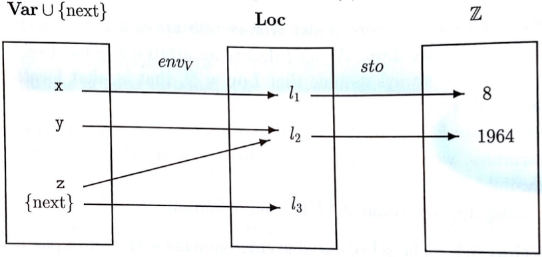
\includegraphics{resources/Images/stoloc.png}
    \caption{Environment-store model illustration \cite{stoloc}}
    \label{fig:Env}
\end{figure}

The following tables are the big step semantics of \lang{}.

\begin{table}[H]
\begin{adjustbox}{center}
\begin{tabular}{|c|c|}
\hline
\vspace {0.1pt} & \\
Num             &   \hbox{\Large \(env_V\, \vdash \langle n\: ,\ sto \rangle \rightarrow_a (v\: ,\ sto') \)\normalsize\(\quad \textbf{if}\ N\llbracket n \rrbracket = v  \)}  \vspace{0.1pt} \\ \hline 
\vspace {0.1pt} & \\  
Var             & \hbox{\Large \(env_V\, \vdash \langle x\: ,\ sto \rangle \rightarrow_a (v\: ,\ sto')\)\normalsize\( \quad \textbf{if} \: \begin{aligned}  env_V\ x=l \\ sto\ l = v \end{aligned} \)} \vspace {0.1pt} \\ \hline
\end{tabular}
\end{adjustbox}
    \caption{Num and var}
    \label{fig:declExp}
\end{table}

\begin{table}[H]
\begin{adjustbox}{center}
\begin{tabular}{|c|c|}
\hline
\vspace {0.1pt} & \\
Var-Decl      & \pbox{20cm}{ \huge \(\frac{env_C\, \vdash \langle D_V\: ,\ env_V']\rangle \rightarrow_{DV}\: (env'_V)}{env_C\, \vdash \langle dcl\ var\ x\ D_V\: ,\ env_V \rangle \rightarrow_{DV}\: env'_V} \)  \\ \\ \\ \normalsize \(  \textbf{where}\quad \: \begin{aligned} l=env_V\ next \\ env_V' = env_V[x \mapsto l][next \mapsto new\ l] \end{aligned} \)} \vspace {0.1pt} \\ \hline
\vspace {0.1pt} & \\
Empty-Var       & \hbox{\Large \(\langle \varepsilon\: ,\ env_V \rangle \rightarrow_{DV} env_V\)} \vspace {0.1pt} \\ \hline

\end{tabular}
\end{adjustbox}
    \caption{Declaration expressions}
    \label{fig:DeclarationExp}
\end{table}

\begin{table}[H]
\begin{adjustbox}{center}
\begin{tabular}{|c|c|}

\hline
\vspace {0.1pt} & \\
Relations 1     &   \pbox{20cm}{\Large \(env\, \vdash \langle a_1\: ,\ sto \rangle \rightarrow_a\: (v_1\: ,\ sto'')\) \\ \huge \(\frac{env\, \vdash \langle a_2\: ,\ sto'' \rangle \rightarrow_a\: (v_2\: ,\ sto')}{env\, \vdash \langle a_1\ op\ a_2\: ,\ sto' \rangle \rightarrow_b\: (\textit{tt}\: ,\ sto')}\)\normalsize\( \quad \begin{aligned} \textbf{if} \ v_1\ op\ v_2 \\ \textbf{where}\  op \in \{=, !=, >, <, >=, <= \}\end{aligned} \)}  \vspace{0.1pt} \\ \hline 
\vspace {0.1pt} & \\  
Relations 2     & \pbox{20cm}{\Large \(env\, \vdash \langle a_1\: ,\ sto \rangle \rightarrow_a\: (v_1\: ,\ sto'')\) \\ \huge \(\frac{env\, \vdash \langle a_2\: ,\ sto'' \rangle \rightarrow_a\: (v_2\: ,\ sto')}{env\, \vdash \langle a_1\ op\ a_2\: ,\ sto \rangle \rightarrow_b\: (\textit{ff}\: ,\ sto')}\)\normalsize\( \quad \begin{aligned} \textbf{if} \ \neg(v_1\ op\ v_2) \\ \textbf{where}\ op \in \{=, !=, >, <, >=, <= \}\end{aligned} \)} \vspace {0.1pt} \\ \hline
\vspace {0.1pt} & \\
Not 1           & \hbox{\huge\(\frac{env\, \vdash \langle b\: ,\ sto \rangle \rightarrow_b\: (\textit{tt}\: ,\ sto')}{env\, \vdash \langle not\ b\: ,\ sto \rangle \rightarrow_b\: (\textit{ff}\: ,\ sto')}\)} \vspace {0.1pt}\\ \hline
\vspace {0.1pt} & \\  
Not 2           & \hbox{\huge\(\frac{env\, \vdash \langle b\: ,\ sto \rangle \rightarrow_b\: (\textit{ff}\: ,\ sto')}{env\, \vdash \langle not\ b\: ,\ sto \rangle \rightarrow_b\: (\textit{tt}\: ,\ sto')}\) } \vspace {0.1pt}\\ \hline
\end{tabular}
\end{adjustbox}
    \caption{Boolean expressions}
    \label{fig:BooleanExp}
\end{table}

\begin{table}[H]
    \centering
    \begin{tabular}{|c|c|}

    \hline
    \vspace {0.1pt} & \\
And 1     & \pbox{20cm}{\Large \(env_V\, \vdash \langle b_1\: ,\ sto \rangle \rightarrow_b (\textit{tt}\: ,\ sto'')\) \\ \huge\(\frac{env_V\, \vdash \langle b_2\: ,\ sto'' \rangle \rightarrow_b\: (v\: ,\ sto')}{env_V\, \vdash \langle b_1\ and\ b_2\: ,\ sto \rangle \rightarrow_b (v\: ,\ sto')}\) } \vspace{0.1pt} \\ \hline 
    \vspace {0.1pt} & \\
And 2     & \hbox{\huge\(\frac{env_V\, \vdash \langle b_1\: ,\ sto \rangle \rightarrow_b (\textit{ff}\: ,\ sto')}{env_V\, \vdash \langle b_1\ and\ b_2\: ,\ sto \rangle \rightarrow_b (\textit{ff}\: ,\ sto')}\)} \vspace{0.1pt} \\ \hline 
    \vspace {0.1pt} & \\
Or 1     & \hbox{\huge\(\frac{env_V\, \vdash \langle b_1\: ,\ sto \rangle \rightarrow_b (\textit{tt}\: ,\ sto')}{env_V\, \vdash \langle b_1\ or\ b_2\: ,\ sto \rangle \rightarrow_b (\textit{tt}\: ,\ sto')}\)} \vspace{0.1pt} \\ \hline 
    \vspace {0.1pt} & \\
Or 2     & \pbox{20cm}{\Large \(env_V\, \vdash \langle b_1\: ,\ sto \rangle \rightarrow_b (\textit{ff}\: ,\ sto'')\) \\ \huge\(\frac{env_V\, \vdash \langle b_2\: ,\ sto'' \rangle \rightarrow_b\: (v\: ,\ sto')}{env_V\, \vdash \langle b_1\ or\ b_2\: ,\ sto \rangle \rightarrow_b\: (v\: ,\ sto')}\) }  \vspace{0.1pt} \\ \hline 
    \end{tabular}
    \caption{Gate expressions}
    \label{fig:GatesExp}
\end{table}

\begin{table}[H]
\begin{adjustbox}{center}
    \begin{tabular}{|c|c|}

    \hline
    \vspace {0.1pt} & \\
Parentheses & \hbox{\huge\(\frac{env_V\, \vdash \langle a\: ,\ sto \rangle \rightarrow_a\: (v\: ,\ sto')}{env_V\, \vdash \langle (a)\: ,\ sto \rangle \rightarrow_a\: (v\: ,\ sto')}\)} \vspace{0.1pt} \\ \hline 
    \vspace {0.1pt} & \\
    \(\begin{aligned}
\textrm{Addition} \\ \textrm{Subtraction} \\ \textrm{Multiplication}\end{aligned}\)  &   \pbox{20cm}{\Large\(env_V\, \vdash \langle a_1\: ,\ sto \rangle \rightarrow_a \: (v_1\: ,\ sto'')\) \\ \huge \(\frac{env_V\, \vdash \langle a_2\: ,\ sto'' \rangle \rightarrow_a\: (v_2\: ,\ sto')}{env_V\, \vdash \langle a_1\ op\ a_2\: ,\ sto \rangle \rightarrow_a \: (v\: ,\ sto')}\)\normalsize\( \quad \textbf{where} \quad op \in \{+,-,\cdot \} \)} \vspace{0.1pt} \\ \hline 
    \vspace {0.1pt} & \\
\(\begin{aligned}\textrm{Division} \\ \textrm{Modulo}\end{aligned}\)   & \pbox{20 cm}{\Large \(env_V\, \vdash \langle a_1\: ,\ sto \rangle \rightarrow_a (v_1\: ,\ sto'')\) \\ \huge \(\frac{env_V\, \vdash \langle a_2\: ,\ sto'' \rangle \rightarrow_a\: (v_2\: ,\ sto')}{env_V\, \vdash \langle a_1\ op\ a_2\: ,\ sto \rangle \rightarrow_a\: (v\: ,\ sto')}\)\normalsize\( \quad \textbf{where} \ \begin{aligned} op \in \{/,mod\} \\ v_2 \neq 0 \end{aligned} \)} \vspace{0.1pt} \\ \hline 
    \vspace {0.1pt} & \\
Unary   & \hbox{\huge\(\frac{env_V\, \vdash \langle a\: ,\ sto \rangle \rightarrow_a\: (v\: ,\ sto')}{env_V\, \vdash \langle -a\: ,\ sto \rangle \rightarrow_a\: (v\: ,\ sto')}\)\normalsize\( \quad \textbf{where} \quad v = -v\)} \vspace{0.1pt} \\ \hline 
    \end{tabular}
\end{adjustbox}
\caption{Arithmetic expressions}
\label{fig:ArithmeticExp}
\end{table}

\begin{table}[H]
\begin{adjustbox}{center}
\begin{tabular}{|c|c|}
\hline
\vspace {0.1pt} & \\
  if 1 &  \pbox{20cm}{\huge\(\frac{env_{VMC}\, \vdash \langle B_1\: ,\ sto'' \rangle \rightarrow (sto'\: ,\ Heap')}{ env_{VMC}\, \vdash \langle if\ b\ then\ B_1\ else\ B_2\ end\: ,\ sto\ \rangle \rightarrow sto'}\) \\ \normalsize\(\textbf{if} \quad env_V\, \vdash \langle b\: ,\ sto \rangle \rightarrow_b (\textit{tt}\: ,\ sto'')\)} \vspace{0.1pt} \\ \hline 
    \vspace {0.1pt} & \\
 if 2 &   \pbox{20cm}{\huge\(\frac{env_{VMC}\, \vdash \langle B_2\: ,\ sto'' \rangle \rightarrow (sto', Heap')}{ env_{VMC}\, \vdash \langle if\ b\ then\ B_1\ else\ B_2\ end\: ,\ sto\ \rangle \rightarrow sto'}\) \\ \normalsize\(\textbf{if} \quad env_V\, \vdash  \langle b\: ,\ sto \rangle \rightarrow_b (\textit{ff}\: ,\ sto'')\)} \vspace{0.1pt} \\ \hline 
    \vspace {0.1pt} & \\
  while 1 &  \pbox{20cm}{\Large \(env_{VMC}\, \vdash \langle B,\: sto'' \rangle \rightarrow (sto'''\: ,\ Heap'')\)\\
  \huge \(\frac{env_{VMC}\, \vdash \langle while\ b\ do\ B\ end\: ,\ sto'''\: ,\ Heap \rangle \rightarrow (sto'\: ,\ Heap)}{env_{VMC}\, \vdash \langle while\ b\ do\ B\ end\: ,\ sto \rangle \rightarrow (sto'\: ,\ Heap')} \) \\ \normalsize\(\textbf{if} \quad env_V\, \vdash \langle b\: ,\ sto \rangle \rightarrow_b (\textit{tt}\: ,\ sto'')\)} \vspace{0.1pt} \\ \hline 
\vspace {0.1pt} & \\
  while 2 &  \pbox{20cm}{\Large\(env_{VMC}\, \vdash \langle while\ b\ do\ B\ end\: ,\ sto\: ,\ Heap \rangle \rightarrow (sto'\: ,\ Heap)\) \\ \normalsize\(\textbf{if} \quad env_V\: ,\ env_C \, \vdash  \langle b\: ,\ sto \rangle \rightarrow_b (\textit{ff}\: ,\ sto')\)} \vspace{0.1pt} \\ \hline 
\vspace {0.1pt} & \\
  \(\begin{aligned} \textrm{for} \\ \textrm{upto 1} \end{aligned}\) &  \pbox{20cm}{\Large\(env_{VMC}\, \vdash \langle for\ x\ upto\ e\ do\ B\ end\: ,\ sto'\: ,\ Heap \rangle \rightarrow (sto'\: ,\ Heap) \) \\  \\ \normalsize \(\textbf{where}\ \begin{aligned} env_V\: ,\ env_C\, \vdash \langle x\: ,\ sto \rangle \rightarrow (v\: ,\ sto) \\ env_V\: ,\ env_C\, \vdash \langle e\: ,\ sto \rangle \rightarrow (v'\: ,\ sto')\\ v > v' \end{aligned}\) } \vspace{0.1pt} \\ \hline 
  \vspace {0.1pt} & \\
  \(\begin{aligned} \textrm{for} \\ \textrm{upto 2} \end{aligned}\) &  \pbox{20cm}{\Large \(env_{VMC}\, \vdash \langle B\: ,\ sto'' \rangle \rightarrow (sto'''\: ,\ Heap'')\) \\ \huge \(\frac{env_{VMC}\, \vdash \langle for\ x\ upto\ n\ do\ B\ end\: ,\ sto'''[l \mapsto v+1]\: ,\ Heap'' \rangle \rightarrow (sto'\: ,\ Heap')}{env_{VMC}\, \vdash \langle for\ x\ upto\ e\ do\ B\ end\: ,\ sto \rangle \rightarrow (sto'\: ,\ Heap')}\) \\ \\ \\ \normalsize\(\quad \textbf{where} \begin{aligned} env_V\: ,\ env_C\, \vdash \langle x\: ,\ sto \rangle \rightarrow (v\: ,\ sto) \\ env_V\: ,\ env_C\, \vdash \langle e\: ,\ sto \rangle \rightarrow (v'\: ,\ sto'') \\ n = N^{-1}[v'] \\ l=env_v\ x \\ v \leq v'  \end{aligned}\)} \vspace {0.1pt} \\ \hline
\end{tabular}
\end{adjustbox}
\caption{Control blocks}
    \label{fig:ControlBlock}
\end{table}

The 'for downto 1-2' are not displayed, as these are identical to 'for upto 1-2' with a few adjustments. The 'upto' operation is replaced with 'downto'. \(v\) has to, in 'downto 1', be less than \(v'\) instead of greater. In 'downto 2', \(v\) has to be greater than or equals \(v'\) instead of less than or equals. Lastly, \(l\) has to, in 'downto 2', map to \(v-1\) instead of \(v+1\). \\


For the sake of readability, \(env_V\: ,\ env_M\) are written as \(env_{VM}\) and \(env_V\: ,\ env_M\: ,\ env_C\) are written as \(env_{VMC}\). The for loop is split into four parts. Two for counting up and two for counting down, although the ones for counting down are, as mentioned above, not displayed. The 'for upto 1' is executed when the value of x is greater than the value of e. This is seen in the side conditions, where the value \(v\) of x, placed in \(sto\), has to be greater than the value \(v'\) of e, placed in \(sto''\), for it to be executed. Since the loop does not run, the storage does not change. 

The 'for upto 2' is executed when the value of x is smaller than the value of e. This is therefore the part that runs the statement in the for loop every time the before-mentioned side condition is true. The first precondition indicates that S is placed in sto''. The reason why this is not just \(sto\) is the fact that it is not necessarily the starting state. This state is executed and placed in \(sto'''\). The second precondition turns the value of e into a numeral with n, which is obtained as \(n = N^{-1}\llbracket v' \rrbracket \), and counts up the location defined by \(l = env_V\ x\) before placing it in \(sto'\).



%in the for upto 2 there is a bit more since this runs more then ones,  the first line \(\langle S,\ Sto''\rangle \rightarrow sto'''\) this say that it will run S, then in the next we count op the \(v\) of location l to \(v + 1\) and then ends, this can run if \(v \leq v'\) where x is stored in \(v\) and e is stored in the \(v'\), it also chance the value \(v'\) to the numerul n \(n=N^{-1}\llbracket v'\rrbracket\) and the location l is equal to the variable x in this enverememt.